\documentclass[binding=0.6cm, LaM]{sapthesis}
\usepackage{microtype}
\usepackage[english]{babel}
\usepackage[utf8]{inputenx}
\usepackage{hyperref}
\usepackage{wasysym}
\usepackage{siunitx}
\hypersetup{pdftitle={My thesis},pdfauthor={Giada Caneva Santoro}}
\usepackage{amsmath, amssymb}
\title{Building a template bank}
\author{Giada Caneva Santoro}
\IDnumber{1490713}
\course{Facolt\`a di Scienze Matematiche Fisiche e Naturali}
\courseorganizer{Corso di Laurea Magistrale in Fisica}
\AcademicYear{2018/2019}
\copyyear{2012}
\advisor{Prof. Francesco Pannarale Greco}
\authoremail{giada.greenday92@gmail.com}
\DeclareUnicodeCharacter{2212}{-}
\begin{document}

\frontmatter
\maketitle
\dedication{Fortsett å gå.}


\tableofcontents

\mainmatter 

\chapter{Introduction}

	More than 100 years ago, Albert Einstein predicted the existence of gravitational waves,
	on the basis of his theory of general relativity.  
	Einstein predicted that the motion of two bodies, such as planets or stars—orbit each other,
	could cause distortions of space-time, gravitational waves.
	These ripples in the fabric of space-time would spread out like the ripples in a pond when a stone is tossed in,
	although their amplitude would be so small that it would be nearly impossible to detect by any technology foreseen at that time.
	It was also predicted that objects moving in an orbit would lose energy for this reason 
	(a consequence of the law of conservation of energy), as some energy would be given off as gravitational waves, 
	although this would be insignificantly small in all but the most extreme cases. 

	Gravitational waves squeeze and stretch anything in their path as they pass by.
	The most powerful gravitational waves are created when objects move at very high speeds. 
	Examples of such things are orbiting pairs of black holes and neutron stars, 
	or massive stars blowing up at the ends of their lives.
	There are four categories of gravitational waves based on what generates them: 
	continuous, compact binary inspiral, stochastic, and burst. 	
	Each category of objects generates a unique or characteristic set of signal 
	that LIGO-Virgo's interferometers can sense, and that researchers can look for in LIGO-Virgo’s data. \\
        The interferometers are designed to detect a specified range of frequencies of gravitational waves,
        which means that they cannot detect objects orbiting at rates that fall outside of this range of frequencies 
        (either too low or too high). \\ 
	During the final moments of the merger of two compact objects such as neutron stars 
	or black holes the emission of gravitational waves is at its peak. The binary loses energy, 
	largely through gravitational waves, and as a result, the two compact objects spiral in towards each other, 
	reaching extreme velocities at the very end of this process. 
	In the final fraction of a second of their merger a significant amount of their mass is converted into gravitational energy, 
	and travel outward as gravitational waves, that potentially fall within the detector’s sensitive range. 
 
	However, the time they spend orbiting in that range of frequencies is typically very brief.
        The masses of the objects involved dictate how long they emit detectable gravitational waves. 
        Heavy objects, like black holes, move through their final inspiral phase much more rapidly than 'lighter' objects, 
        like neutron stars. This means that black-hole merger signals are much shorter than neutron star merger signals.
        For example, the first detection of a gravitational wave signal, GW150914, coming from the a pair of merging black holes, 
	produced a signal just two-tenths of a second long. \\
        In contrast, the first neutron star merger LIGO detected in August 2017 generated a signal over 100 seconds long.
	This first observation was a a remarkable accomplishment: it demonstrated both the existence of binary stellar-mass black hole systems, 
	and the fact that such mergers could occur within the current age of the universe.  
	It also confirmed the last remaining unproven prediction of general relativity and validated 
	its predictions of space-time distortion in the context of large scale cosmic events. 
	Prior to this first detection, gravitational waves had only been inferred indirectly,
        via their effect on the timing of pulsars in binary star systems.
	This event  marked the beginning of a new era of gravitational-wave astronomy, 
	which would enable observations of violent astrophysical events that were not previously possible, 
	and potentially allow the direct observation of the birth of the universe.


%----------------------------------------------------------------------------------------------------------------------------------------------------------------------------------------------------------
\chapter{Gravitational Wave Detection Principles}
\section{Gravitational waves in linearized gravity}

\subsection{Weak-field metric}

	In 1915, Albert Einstein presented his general theory of relativity  which describes 
	how mass distorts spacetime and in turn how spacetime dictates how masses flow through it.
	The classical Newtonian notion of gravity ,which stated that gravity arises from an 
	action at a distance, was replaced with a geometric interpretation of the Universe, 
	the spacetime continuum: it can be regarded as a fabric and it can be curved 
	by the mass of an object. \\
	Masses moving on this curved spacetime fabric will then be perceived as gravity.
	In general relativity, space-time is regarded as a four-dimensional manifold 
	with a Lorentzian metric, and gravity is a manifestation of the manifold’s curvature. \\
	The spacetime curvature is associated with the stress-energy tensor 
	of matter fields through the Einstein’s field equations:

		\begin{equation}
		G_{\mu\nu} \equiv R_{\mu\nu}  - {1 \over 2}g_{\mu\nu}R = {8\pi G_{N} \over {c^4}}T_{\mu\nu} 
		\end{equation}

	Where $G_{\mu\nu} $ is the Einstein tensor, $T_{\mu\nu} $ is the stress-energy 
	tensor of matter-fields and $ G_{N}$ is Newton’s gravitational constant. \\
	General relativity predicts that gravity is mediated by a new type of radiation: gravitational radiation. 

	In 1916 Einstein found the weak-field solutions to general relativity had wave-like solutions, gravitational waves.
	Gravitational waves that compose gravitational radiation are ripples in the fabric of spacetime, 
	which periodically lengthen and shorten space, and speed up and slow down time.
 	To study the properties of gravitational waves, it is instructive to first study them 
	in situations where the gravitational fields are weak.
	In the so-called weak-field approximation, one can view the metric as the Minkowski metric 
	with a small perturbation: it is required to expand the Einstein equations around the flat-space metric,
	considering as a perturbation on the space-time of special relativity.
	Letting $ x_\mu = (t, x, y, z)$ denote the time and space coordinates, 
	we can write the proper distance between events $x_{\mu}$ and $x_{\mu} + dx_{\mu}$ as
		
		\[
		ds^2 = g_{\mu\nu}dx^{\mu}dx^{\nu} \approx (\eta_{\mu\nu} + h_{\mu\nu})dx_{\mu}dx_{\nu}. \hspace*{2cm}\|h_{\mu\nu}\|\ll 1
		\]

	Here $\eta_{\mu\nu} = diag(-1,1,1,1)$ is the usual Minkowski metric and $h_{\mu\nu}$ 
	represents the linearised gravitational field. \\
	The metric perturbation is referred to as  $h_{\mu\nu}$: it encapsulates gravitational waves, 
	but contains additional, non-radiative degrees of freedom as well; $\|h_{\mu\nu}\|$ means
	“the magnitude of a typical non-zero component of $h_{\mu\nu}$”. \\ 
	The condition $\|h_{\mu\nu}\|\ll 1$ requires both the gravitational field to be weak, 
	and in addition constrains the coordinate system to be approximately Cartesian.  
	In linearized gravity, the smallness of the perturbation means that only terms which are linear in $h_{\mu\nu}$ are considered;
	higher order terms are discarded. As a consequence, indices are raised and lowered using the flat metric. \\
	The metric perturbation $h_{\mu\nu}$ transforms as a tensor under Lorentz transformations, 
	but not under general coordinate transformations: since the numerical values of the components
	of a tensor depend on the reference frame, there exists a reference frame where 
	the linearisation of the gravitational field holds on a sufficiently large region of the spacetime. \\
	The Einstein field equations are covariant under general coordinate transformations

		\begin{equation}
		x^{\mu} \rightarrow x^{\mu ‘}(x)
		\end{equation}

	So that the metric transforms as

		\begin{equation}
		g_{\mu\nu} \rightarrow g_{\mu' \nu'} = x^{\rho},_{\mu'}x^{\sigma},_{\nu'}g_{\rho \sigma}
		\end{equation}

	This means that one is free to choose a convenient coordinate system without 
	altering the physical predictions of the field equations.
	Choosing a reference frame breaks the invariance of general relativity under 
	coordiante trasformations but it also erases spurious degrees of freedom. \\
	However,after choosing a frame where the field is linearised, 
	a residual gauge symmetry remains. \\
	Under infinitesimal coordinate transformations
                 \[
		x_{\mu} \rightarrow x_{\mu} + \xi_{\mu}
                \]

	using the transformation law of the metric, to lowest order $h_{\mu\nu}$ transforms as
			
		\[
		h_{\mu\nu} \rightarrow h_{\mu\nu} - \partial_{\mu}\xi_{\nu} - \partial_{\nu}\xi_{\mu}
		\]


\subsubsection{Linearising the Einstein field equations}

	All the fundamental quantities in the field equations need to be computed in order to linearise the theory.
	Rather than working with the metric perturbation, changing notation and using the trace-reversed perturbation 
	makes the computation more compact and cleaner. Defining
	
		\begin{equation}
		{\bar h}_{\mu\nu} = h_{\mu\nu} - {1 \over {2}}\eta_{\mu\nu}h  
		\end{equation}

	and the trace
	
		\begin{equation}
		h = \eta^{\mu\nu}h_{\mu\nu}
		\end{equation}

	expressing the trace-reversed field:

		\begin{equation}
		h_{\mu\nu} = {\bar h}_{\mu\nu} + {1 \over {2}}\eta_{\mu\nu}{\bar h}
		\end{equation}

	The Rienmann tensor constructed in linearised theory is given by

		\begin{align}
		R^{\mu}_{\nu\rho\sigma} &= \partial_{\rho} \Gamma^{\mu}_{\nu\sigma} - \partial_{\sigma}\Gamma^{\mu}_{\nu\rho}  \\
				       &= {1 \over 2} (\partial_{\rho}\partial_{\nu}h^{\mu}_{\nu\rho} + \partial_{\sigma}\partial^{\mu}h^{\nu\rho} - \partial_{\rho}\partial^{\mu}h^{\nu\sigma} - \partial_{\					     \sigma}\partial_{\nu}h^{\mu}_{\rho})
		\end{align}

	From this, the Ricci tensor takes the form

		\begin{equation}
		R_{\mu\nu} = R^{\rho}_{\mu\rho\nu} = {1 \over 2}(\partial_{\rho}\partial_{\nu}h^{\rho}_{\mu} + \partial^{\rho}\partial_{\mu}h_{\nu\rho} - \square h_{\mu\nu} - \partial_{\mu}\partial_{\nu}h)
		\end{equation}

	The curvature scalar is obtained contracting once more:

		\begin{equation}
		R = R^{\mu}_{\mu} = (\partial_{\rho}\partial^{\mu}h^{\rho}_{\mu} - \square h)
		\end{equation}

	Combining all together the Einstein tensor can be expressed as
	
		\begin{equation}
		G_{\mu\nu} = {1 \over 2}(\partial_{\rho}\partial_{\nu}h^{\rho}_{\mu} + \partial^{\rho}\partial_{\mu}h_{\nu\rho} - \square h_{\mu\nu} - \partial_{\mu}\partial_{\nu}h - \eta_{\mu\nu}\partial_{\rho}\partial^{\sigma}h^{\rho}_{\sigma} + \eta_{\mu\nu}\square h)
		\end{equation}

	Substituting the metric perturbation $h_{\mu\nu}$  with the $trace-reversed$ perturbation ${\bar h}_{\mu\nu}$ and expandig, 
	the linerised Einstein equations assume the  compact form:

		\begin{equation}
		\square {\bar h}_{\mu\nu} + \eta_{\mu\nu}{\partial}^{\rho}{\partial}^{\sigma}{\bar h}_{\rho\sigma} - {\partial}^{\rho}{\partial}^{\nu}{\bar h}_{\mu\rho} - {\partial}^{\rho}{\partial}^{\mu}{\bar h}_{\nu\rho} = - {{16\pi G_{N}} \over {c^4}}T_{\mu\nu}.
		\end{equation}

	The linearised equations of motion are gauge-invariant, and the gauge freedom can
 	be used to simplify the form of the field equations.
 	In the Lorentz family of gauges, choosing the harmonic gauge $ \partial_{\mu}h_{\mu\nu} = 0 $, 
	reduces the Einstein equations to a simple wave equation that relates the trace-reversed field
 	to the stress energy tensor:

		\begin{equation}
		\square {\bar h}_{\mu\nu} =({\partial^2 \over {\partial t^2} } - {\partial^2 \over {\partial x^2}}  - {\partial^2 \over {\partial y^2}}  -  {\partial^2 \over {\partial z^2}}) {\bar h}_{\mu\nu} = -{{16\pi G_{N}} \over {c^4}}T_{\mu\nu}. 
		\end{equation}

	By imposing the harmonic gauge one has chosen the coordinates in such a way that for a single plane wave 
	(or a superposition of plane waves with their wave vectors pointing in the same direction),
	the GW polarisations are perpendicular to the direction of propagation.

	The harmonic gauge gives four conditions, that reduce the 10 indipendent component of the symmetric 4x4 matrix 
	$h_{\mu\nu}$ to six indipendent component, so it does not fix the gauge completely,
	leaving 4 additional components free to be gauge-fixed.
	If the metric perturbation is not in the harmonic gauge, by making an infinitesimal coordinate transformation

		\begin{equation}
		{\bar h}_{\mu\nu} \rightarrow {\bar h}_{\mu’\nu’}  = {\bar h}_{\mu\nu}  - \xi_{\mu,\nu} -\xi_{\nu,\mu} + \eta_{\mu\nu}\xi^{\rho}_{,\rho}
		\end{equation}

	and applying the harmonic gauge condition

		\begin{equation}
		{\bar h}_{\mu’\nu’,} ^{\nu’} = {\bar h}_{\mu\nu,} ^{\nu} - \xi_{\mu,\nu}^{\nu}
		\end{equation}

	Therefore any metric perturbation can be put into an harmonic gauge by making an infinitesimal 
	coordinate transformation that satisfies

		\begin{equation}
		{\bar h}_{\mu\nu,} ^{\nu} = \xi_{\mu,\nu}^{\nu}
		\end{equation}

	This is a wave equation that always admits a solution, thus one can always achieve the harmonic gauge. \\
	Outside the source where $T_{\mu\nu} = 0$

		\begin{equation}
		\square {\bar h}_{\mu\nu} = 0
		\end{equation}

	In vacuum spacetimes which are asymptotically flat ($h_{\mu\nu} \rightarrow 0$ as $r \rightarrow 0$), 
	along with choosing the harmonic gauge, the metric perturbation can be greatly simplified using
	the residual gauge freedom within the harmonic gauge class. \\
	The transverse-traceless gauge, $TT$-gauge, can be obtained by choosing the components of the metric tensor $h_{\mu\nu}$,
	so that only the ones on the plane orthogonal to the direction of propagation (transverse) 
	are different from zero, this results in $h_{\mu\nu}$ being traceless:

		\begin{equation}
		h^{0\mu} = 0 \hspace*{0.5cm}  h^{i}_i = 0  \hspace*{0.5cm}   {\partial}^jh_{ij} = 0
		\end{equation}

	By imposing the harmonic gauge, the 10 degrees of freedom of the symmetric matrix $h_{\mu\nu}$ 
	have reduced to six degrees of freedom, and the residual gauge freedom,
	associated to the four function $\xi^{\mu}$, has further reduced these to just two degrees of freedom, 
	which corrispond to the two possible polarization states of the gravitational wave. \\
	Equation (2.17) has plane wave solutions, $h_{\mu\nu}^{TT}(x)=e_{ij}(k)e^{ikx}$ with 
	$k^{\mu}=(w/c,k)$ and $w/c=|k|$. The tensor $e_{ij}(k)$ is called the polarization tensor. \\

	In vacuum spacetimes, a plane gravitational wave with a given wave-vector $k$ is characterized 
	by two functions $h_+$ and $h_{\times}$, while the remaining components can be set to zero by
	choosing the transverse-traceless gauge. \\
	Choosing $n$ along the z axis:

		\begin{equation} 
		h_{\mu\nu}^{TT} = 
		\begin{bmatrix}
		0 & 0 & 0 & 0 \\
		0 & h_{+} & h_{\times} & 0 \\
		0 & h_{\times} & -h_{+} & 0 \\
		0 & 0 & 0 & 0 
		\end{bmatrix}cos[w(t-z/c)]
		\end{equation}

\subsubsection{Geodesic equation and geodesic deviation}

	The usual notion of “gravitational force” disappears in general relativity, replaced instead 
	by the idea that freely falling bodies follow geodesics in spacetime.
	Geodesics are the curved-space equivalents of straight lines, which can be found by 
	parallel transporting the tangent vector of a curve.
	Given a spacetime metric $g_{\mu\nu}$ and a set of spacetime coordinates $x^{\mu}$, 
	geodesic trajectories are given by the equation:

		\begin{equation}
		{{d^2x^{\mu}}\over{d\tau^2}} + \Gamma_{\nu\rho}^{\mu}(x){{dx^{\nu}}\over{d\tau}}{{dx^{\rho}}\over{d\tau}} = 0 \hspace*{2cm} m \neq 0
		\end{equation}

		\begin{equation}
		{{d^2x^{\mu}}\over{d\lambda^2}} + \Gamma_{\nu\rho}^{\mu}(x){{dx^{\nu}}\over{d\lambda}}{{dx^{\rho}}\over{d\lambda}} = 0 \hspace*{2cm} m = 0
		\end{equation}

	which is the classical equation of motion of a test mass in the curved background described 
	by the metric $g_{\mu\nu}$, in the absence of external non gravitational force and where $m$ is the mass
	of the object, $\tau$ represents the proper time given by $d\tau^2 = -ds^2$, 
	and $\lambda$ is some affine parameter on the geodesic.
	In a flat spacetime, two straight lines that are initially parallel to each other will remain parallel. \\
	In a curved spacetime, geodesics do not satisfy this property.
	Instead, two nearby geodesics, separeted by $\zeta^{\mu}$, follow the geodesic deviation equation
		
		\begin{equation}
		{{D^2\zeta^{\mu}}\over{D\tau^2}} = -R^{\mu}_{\nu\rho\sigma}\zeta^{\rho}{{dx^{\nu}}\over{d\tau}}{{dx^{\sigma}}\over{d\tau}}
		\end{equation}

	where $D/D\tau$ is defined as

		\begin{equation}
		{{DV^{\mu}}\over{D\tau}} \equiv {{dV^{\mu}}\over{d\tau}} + \Gamma^{\mu}_{\nu\rho}V^{\nu}{{dx^{\rho}}\over{d\tau}}
		\end{equation}

	and denotes the covariant derivative along a curve that is parameterised by $\tau$. 
	The geodesic deviation equation describes the change in separation $\zeta^{\mu}$ between two nearby geodesic.
	As the Rienmann tensor describes the tidal forces caused by the gravitational field, 
	the geodesic deviation equation shows that these tidal forces can be considered as deviations of nearby geodesics.

\subsection{Interaction of Gravitational waves with test masses}

	To understand how gravitational waves interact with the detectors, mirrors in the case of the interferometric detectors, 
	it's necessary to use the geodesic equation and the geodesic deviation equation, which are also important tools 
	for understanding the physical meaning of a given gauge choice. \\
	In fact the physics must be invariant under coordinate trasformations but GWs and the detector description's depend on the chosen reference frame.

\subsubsection{Transverse-traceless gauge}
	Gravitational waves take a particularly simple form in the $TT$-gauge 
	and choosing a gauge is equivalent to selecting a reference frame. 
	Consider a test mass initially at rest at $\tau = 0$. The geodesic equation then becomes

		\begin{equation}
		{{dx^i}\over{d\tau^2}} = -[\Gamma^i_{\nu\rho}{{dx^{\nu}}\over{d\tau}}{{dx^{\rho}}\over{d\tau}}]_{\tau=0} \\ 
		= - [ \Gamma^i_{00}({{dx^0}\over{d\tau}})^2]_{\tau=0}
		\end{equation}

	by assumption
		
		\begin{equation}
		{{dx^i}\over{d\tau}} = 0 \hspace*{2cm} at \hspace*{0.5cm}\tau = 0
		\end{equation}

	since the mass is initially at rest. Expanding to first order in $h_{\mu\nu}$, 
	the Christoffel symbol $\Gamma^i_{00}$ vanishes in the TT gauge

		\begin{equation}
		\Gamma^i_{00} = {1 \over {2}}(2\partial_{0}h_{0i} - \partial_i h_{00})
		\end{equation}

	because both $h_{00}$ and $h_{0i}$ are set to zero by the gauge condition. 
	Therefore, if at time $\tau = 0$, $dx^i/d\tau$ is zero, remains zero at all times, 
	because its derivatives also vanishes. \\
	This shows that if two test masses are initially separated by a coordinate separation of $x^i$ in the TT frame, 
	and are at rest with respect to each other, they will remain at this separation. \\
	Overall, it seems that a GW has no influence on the geodesic or on the deviation of geodesics.
	In other words, in the TT gauge the coordinate location of a slowly moving, freely falling body is unaffected 
	by the GW because the coordinates move with the waves.
	The TT gauge illustrates that, in general relativity, the physical effects are not expressed by what happens 
	to the coordinates since the theory is invariant under coordinate transformations:
	the position of test masses doesn't change because the freedom of gauge allowed to define the coordinates 
	in such a way that they don't change.
	Physical effects can instead be found monitoring proper distances, or proper times.

	In fact the GWs cause the proper separation between two freely falling particles to oscillate, 
	even if the coordinate separation is constant. Consider two spatial freely falling particles, 
	located at $z = 0$, and separated on the x axis by a coordinate distance $L_c$. \\
	Consider a GW in TT gauge that propagates down the z axis, $h^{TT}_{\mu\nu}(t,z)$. 
	The proper distance L between the two particles in the presence of the GW is given by

		\begin{align}
		L & = \int^{L_c}_{0}{dx\sqrt{g_{xx}}} = \int^{L_c}_{0}dx\sqrt{1 + h^{TT}_{xx}(t,z=0)} \\
		& \simeq \int^{L_c}_{0}{dx[1 + {1 \over 2}h^{TT}_{xx}(t,z=0)]} \\
		&= L_c[1 + {1 \over 2}h^{TT}_{xx}(t,z=0)]
		\end{align}

	Therefore, the proper distance expands and shrinks periodically,with a fractional length change $\delta L/L$ given by

		\begin{equation}
		{{\delta L}\over{L}} \simeq {1 \over 2} h_{xx}^{TT}(t,z=0)
		\end{equation}

	Even though this result is calculated in the TT gauge, it is indeed gauge indipendent;
	$h_{xx}^{TT}$ acts as a strain, a fractional length change.
	Because the time that light travels between the two test masses is related to the proper distance,  
	which directly relates to the accumulated phase measured by laser interferometric GW observatories,
	GWs leave an imprint on the time it takes for a photon to make a round trip. 
	Consequently, interferometers can potentially measure these imprints by measuring the length difference between
	their arms. The “extra” phase $\delta \phi$ (if $L \ll \lambda$ so that the metric perturbation 
	does not change value very much during a light travel time) accumulated by a photon that travels
	down and back the arm of a laser interferometer in the presence of a GW is $\delta \phi = 4\pi \delta L \lambda$, 
	where $\lambda$ is the photon’s wavelength and $\delta L$ is the distance
	the end mirror moves relative to the beam splitter.


\subsubsection{Local proper reference frame}

	Since positions in a lab are not marked by test particles,  
	the $TT$ frame is not very practical. 
	The preferred reference frame is the proper detector frame 
	in which the test particle is free to move because of a passing gravitational wave. 
	The path of a test particle can then be described by Newtonian equations of motion in terms of forces. 
	There are terms proportional to the Riemann curvature tensor from the gravitational field of the Earth 
	but also terms from static gravitational forces, Coriolis forces, etc. 
	In order to leave only the part proportional to the Riemann tensor, 
	earth-based detectors look for higher frequency gravitational waves, 
	as gravitational waves with low frequencies are comparable with slowly varying Newtonian noises. 
	The acceleration in the $z$-direction due to Earth’s gravity can be dealt with suspension systems 
	allowing the test mass to act as if they were in a freely falling frame in the $x - y$ plane. 

	Consider a detector capable of measuring changes in the proper distance, e.g. an interferometer, 
	with a characteristic size that is much smaller than the characteristic wavelength of the GW.
	In this case, one can approximate the entire detector to be in a near local Lorentz frame  
	(freely falling frame), even in the presence of GWs. This coordinate system is defined by the requirements

		\begin{equation}
		z^i(\tau) = 0, \hspace*{2cm} g_{ab}(t, 0) = \eta_{ab}, \hspace*{2cm} \Gamma^a_{bc}(t,0) = 0,
		\end{equation}

	which imply that the metric has the form

		\begin{equation}
		ds^2 \approx -dt^2 + \delta_{ij}dx^i dx^j + O({{x^ix^j}\over{L^2_B}})
		\end{equation}

	where $L^2_B$ denotes the typical variation scale of the metric.
	Consider now the proper distance between the two geodesics, $\zeta^i$, 
	to understand how the GWs influence these two test masses the geodesic deviation equation is calculated as

		\begin{equation}
		{{d^2\zeta^{\mu}}\over{d\tau^2}} + 2\Gamma^{\mu}_{\nu\rho}{{dx^{\nu}}\over{d\tau}}{{dx^\rho}\over{d\tau}} + \zeta^{\sigma}\Gamma^{\mu}_{\nu\rho,\sigma}{{dx^{\nu}}\over{d\tau}}{{dx^{\rho}}\over{d\tau}} = 0
		\end{equation}

	Assuming the two test masses are moving non-relativistically, $dx^i/d\tau$ can be neglected compared to $dx^0/d\tau$.
	Furthermore, the term proportional to $\Gamma^{\mu}_\nu\rho{}$ is negligible compared to other terms in a near LLF. Hence,

		\begin{equation}
		{{d^2\zeta^{\mu}}\over{d\tau^2}} + \zeta^{\sigma}\Gamma^{i}_{00, \sigma}({{dx^0}\over{d\tau}})^2 = 0
		\end{equation}

	Further simplifying $\zeta^{\sigma}\Gamma^{i}_{00, \sigma} \approx \zeta^{j}\Gamma^{i}_{00, j}$

		\begin{equation}
		{{d^2\zeta^{\mu}}\over{d\tau^2}} + \zeta^{j}\Gamma^{i}_{00,j}({{dx^0}\over{d\tau}})^2 = 0
		\end{equation}

	But in the LLF, $R^i_{0j0} = \Gamma^i_{00,j} - \Gamma^i_{0j,0} = \Gamma^i_{00,j}$ and therefore

		\begin{equation}
		{{d^2\zeta^{\mu}}\over{d\tau^2}} + R^i_{0j0} \zeta^j({{dx^0}\over{d\tau}})^2 = 0
		\end{equation}

	Because $dx^0/d\tau \approx 1$, one can approximate $\tau \approx t$:

		\begin{equation}
		{\ddot \zeta}^j = - R^i_{0j0}\zeta^j
		\end{equation}
	
	The key quantity entering into the equation, the Rienmann tensor, is gauge invariant in linearized theory, 
	it can be evaluated in any convenient coordinate system.
	The expression for the Rienmann tensor in terms of the TT gauge metric perturbation $h_{ij}^{TT}$

		\begin{equation}
		R^i_{0j0} = R_{i0j0} = - {1 \over 2}{\ddot h}_{ij}^{TT}
		\end{equation}

	Substituting into the previous equation, the geodesic deviation equation in the proper detector frame takes the form

		\begin{equation}
		{\ddot \zeta}^i = {1 \over 2}{\ddot h}_{ij}^{TT}\zeta^j
		\end{equation}

	which can be interpreted as if the influence of a GW in a near LLF resembles a Newtonian force.
	In general directions, the proper distance is given by

		\begin{equation}
		s = \sqrt{L^2 + h_{ij}(t)L_{i}L_{j}}
		\end{equation}

	where $L_i$ denotes the spatial separation between two test masses and $L$ the associated coordinate distance.
	In the given metric for the proper reference frame, the proper distance is just $|L| = \sqrt{L_iL_j}$ up to fractional errors; 
	since the only detectors taken in consideration are those
	with $L \ll \lambda$, these errors are smaller than the fractional distance changes caused by the GW.
	Therefore $|L|$ is simply identified as the proper separation. The ideal equation for analyzing an interferometric GW detector is

		\begin{equation}
		{\ddot L}^i = {1 \over 2}{\ddot h}_{ij}^{TT}L^j
		\end{equation}


\subsubsection{Ring of test masses}

	The effects of gravitational waves cannot be seen in isolated bodies. 
	This is a result of the fact that a single test mass, in a frame freely falling with it, 
	will remain at rest. At least two test masses are required to measure the effects of gravitational waves. 
	This is also the case when one wants to measure any curvature of spacetime.
	Consider a ring of test masses in the $(x, y)$ plane of a proper detector frame, initially at rest, centred at $z = 0$, 
	and a GW travelling in the $z$-direction.
	This situation restricts the attention to the $(x,y)$ plane alone, because $h_{ij}^{TT}$ is transverse to the propagation direction, 
	so the GW will only have influence in the plane of the test masses:
	the only non zero compontents of the metric perturbation are

		\begin{equation}
		h_{xx}^{TT} = - h_{yy}^{TT} = h_{+} \hspace*{3cm} h_{xy}^{TT} = h_{yx}^{TT} = h_{\times}
		\end{equation}

	where $h_{+}(t-z)$ and $h_{\times}(t-z)$ are the two polarization components, which are indipendent and can be considered separately.
	For the plus polarization at $z=0$ and initial conditions $h_{ij}^{TT} = 0$ at $t=0$:

		\begin{equation}
		h_{ab}^{TT} = 
		\begin{bmatrix}
		1  & 0 \\
		0 &  -1 \\
		\end{bmatrix} 
		h_{+}\cos \omega t
		\end{equation}

	If the displacement between geodesics is $\zeta_a (t) = (x_0 + \delta x(t), y_0 + \delta y(t))$, then of $\zeta_a (t)$ is

		\begin{equation}
		\delta {\ddot x} = - {{h_{+}} \over 2} (x_0 + \delta x) \omega ^2 \sin \omega t
		\end{equation}

		\begin{equation}
		\delta {\ddot y} =  {{h_{+}} \over 2} (y_0 + \delta y) \omega ^2 \sin \omega t
		\end{equation}

	Assuming that the perturbations are $O(h)$, and thus small compared to the unperturbed locations, $\delta x$ and $\delta y$ can be neglected.
	The integrations gives the deviations caused by the plus polarisations:

		\begin{equation}
		\delta x(t) =  {{h_{+}} \over 2} x_0 \sin \omega t
		\end{equation}

		\begin{equation}
		\delta y(t) = - {{h_{+}} \over 2} y_0  \sin \omega t
		\end{equation}

	Similarly, for the cross polarization at $z=0$ and initial conditions $h_{ij}^{TT} = 0$ at $t= 0$, the situation is described by the equations
		
		\begin{equation}
		\delta x(t) =  {{h_{\times}} \over 2} y_0 \sin \omega t
		\end{equation}

		\begin{equation}
		\delta y(t) =  {{h_{\times}} \over 2} x_0  \sin \omega t
		\end{equation}
		
	This set of equations describes the changes in the x and y components for a passing gravitational wave.
	The plus polarization alternately stretches and compresses the ring of test masses in the x and y directions, 
	while the cross polarization exhibits the same behavior rotated by $\ang{45}$ in the x - y plane.

		\begin{figure}
		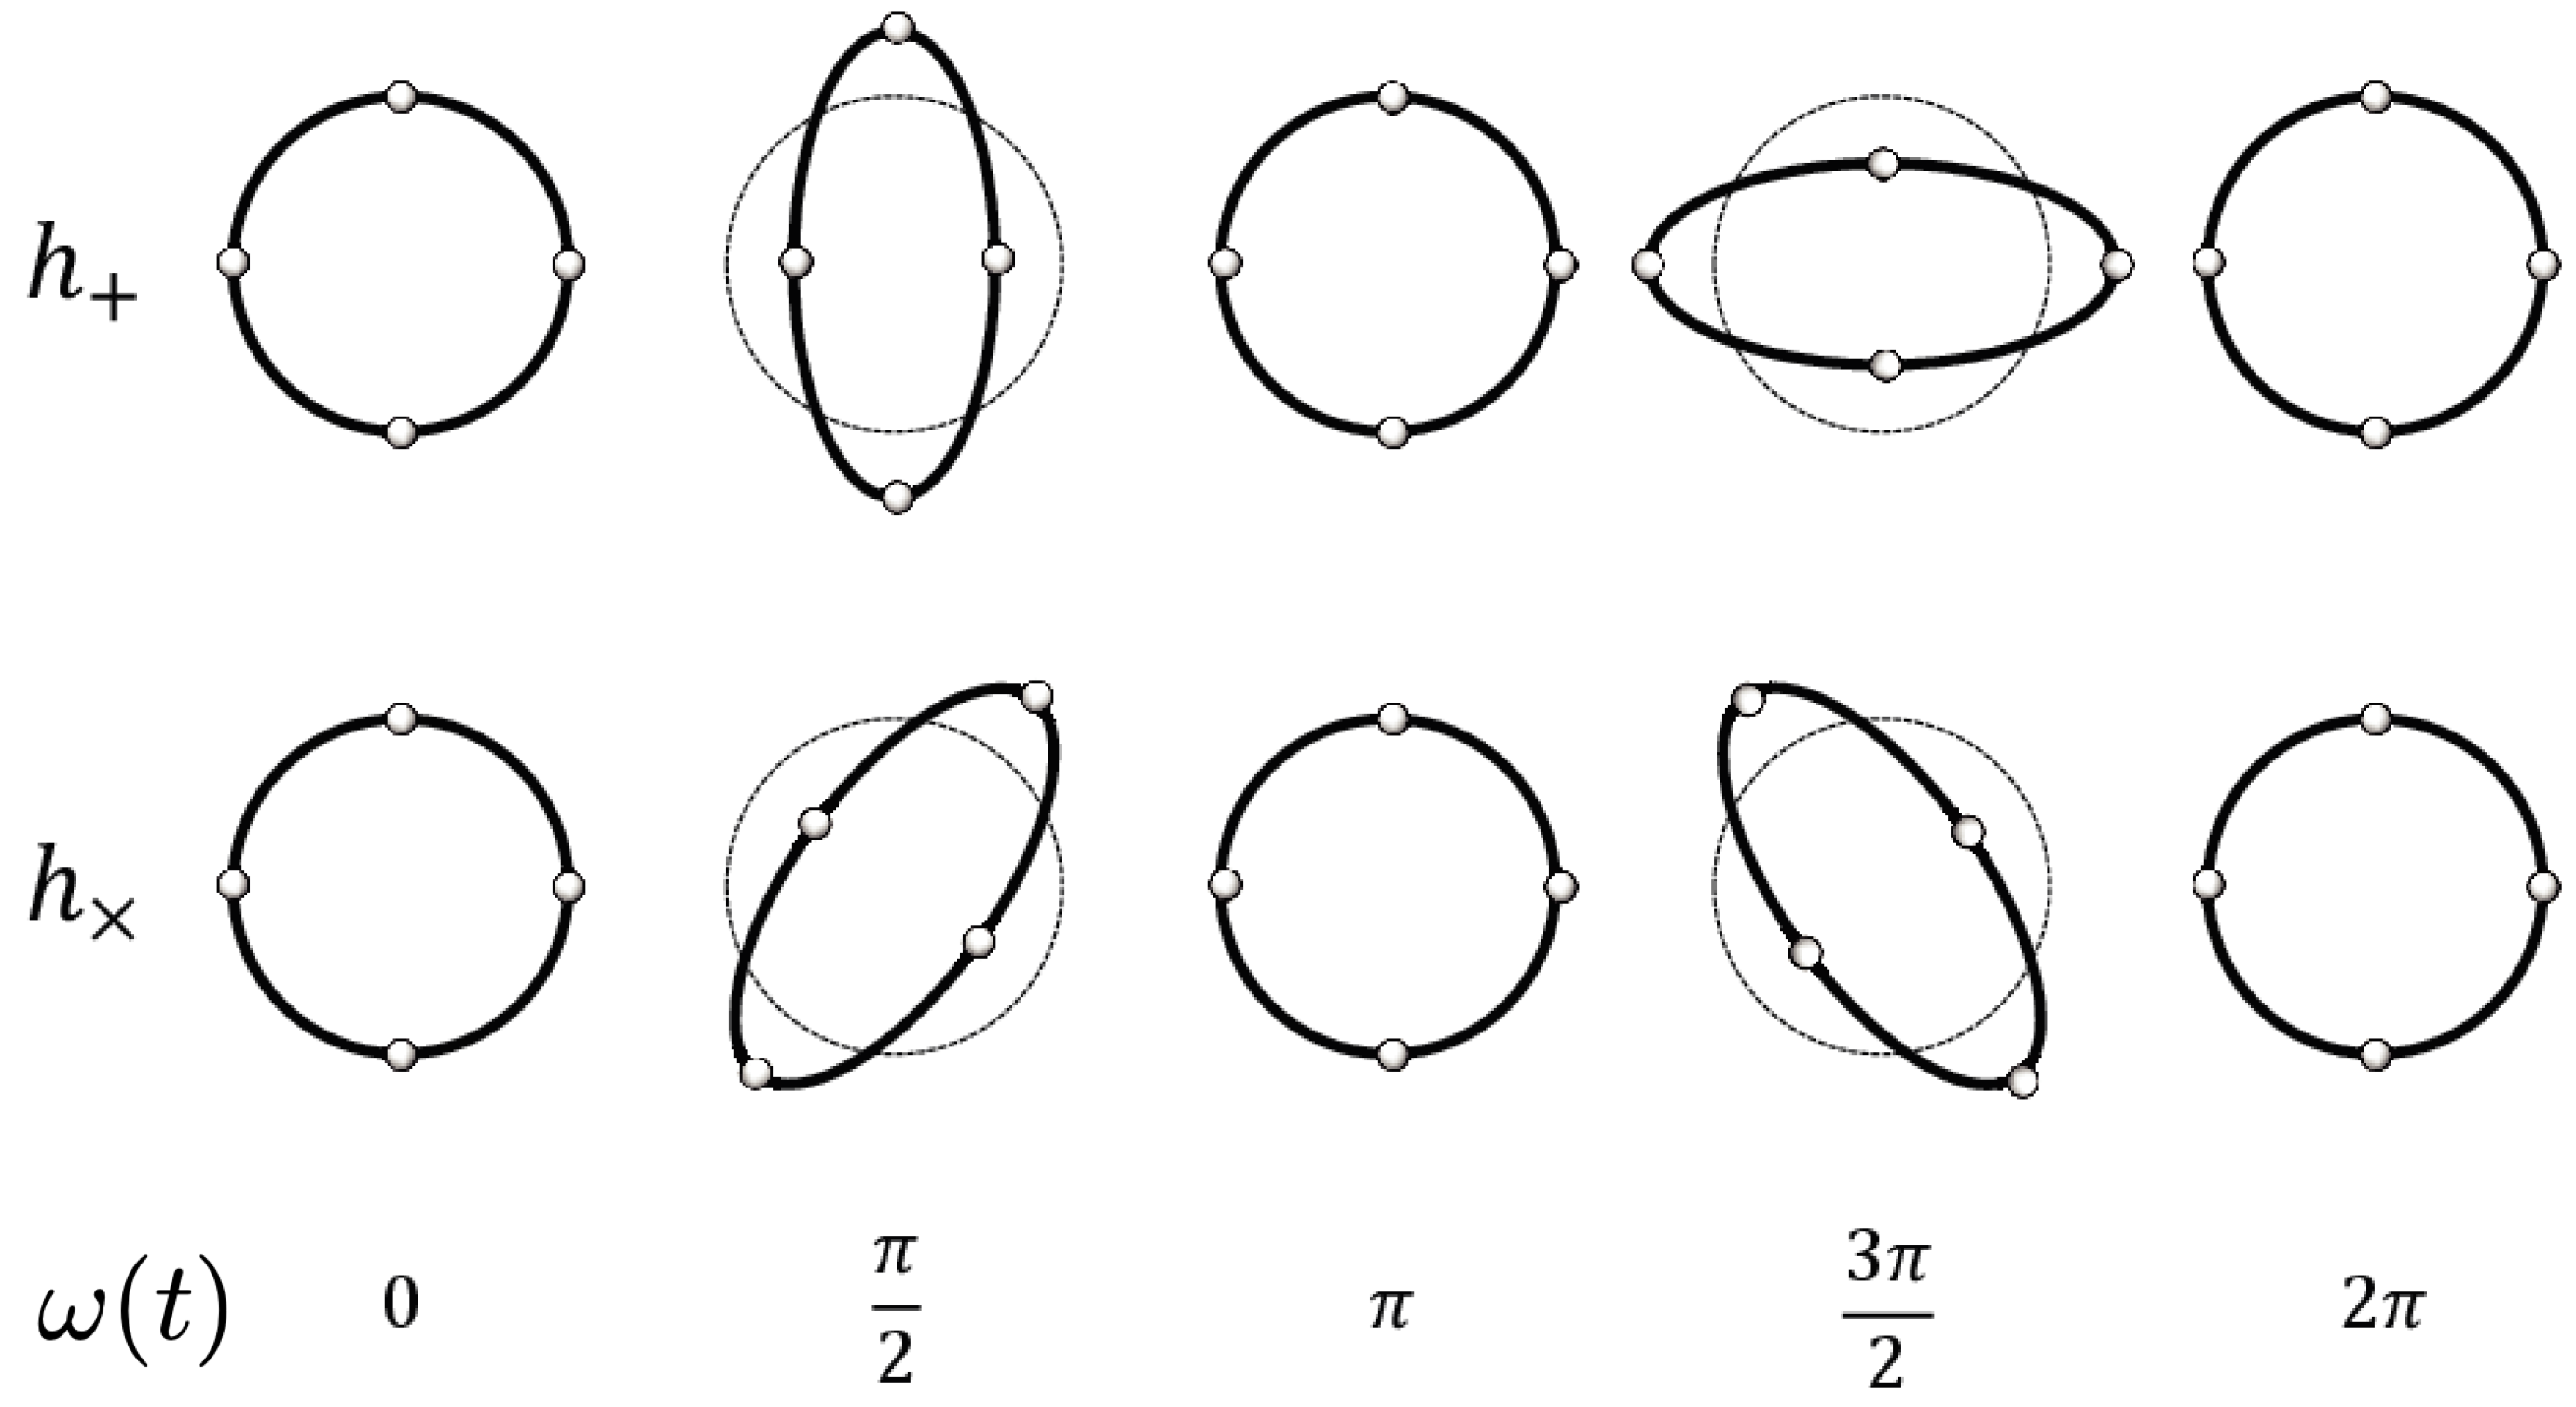
\includegraphics[scale=1]{ring}
		\centering
		\caption{The effects of plus and cross polarization on a ring of test masses. 
			 The plus polarization alternately compresses and stretches the x- and y-separations.
			 The cross polarization has the same effect only rotated by  $\ang{45}$.}
		\label{fig:ring}
		\end{figure}

\subsection{Beam pattern functions}

        Interferometers are sensitive to the relative difference between two distances, the so-called strain.
        Suppose we have an interferometer with its arms pointing along the unit vectors $u^i$ and $v^i$. The strain $h(t)$ is given by

                \begin{equation}
                h(t) = {1 \over 2} (h_{ij}u^iu^j - h_{ij}v^iv^j) = D^{ij}h_{ij}(t)
                \end{equation}

        where $D^{ij}$ is referred to as the detector tensor and is given by

                \begin{equation}
                D^{ij} = {1\over 2} (u^iu^j -v^iv^j)
                \end{equation}

        As the expression for $h(t)$ is linear in $h_{+}$ and $h_{\times}$, one can also write

                \begin{equation}
                h(t) = F_{+}h_{+} (t) + F_{\times}h_{\times}(t)
                \end{equation}

        where $F_{+,\times}$ are called the beam pattern functions. Suppose we have a detector
        with arms that are perpendicular to each other, one pointing in the x-direction and the other
        in the $y$-direction in a Cartesian coordinate system. This detector frame, denoted by $(x,y,z)$,
        is generally different from the GW coordinate system, denoted by $(x^\prime,y^\prime,z^\prime)$, where the source
        is conveniently described. To account for such a difference, we first note that when the plus
        and cross polarisations are not equal in strength, we can rotate the coordinate system by
        an angle $\psi$ around the $z^\prime$ axis so that the $x^\prime$ and $y^\prime$ axes
        coincide with the mayor and minor axis of the associated ellipse.
        In going from the GW frame to the detector frame, we can rotate the GW frame by
        an angle $\theta$ around the $x^\prime$ axis and an angle $\phi$ around the $z^\prime$ axis,
        where the angles $(\theta, \phi)$ denote the direction of propagation of the GW in the detector frame.
        Applying these three rotations, the beam pattern functions for a detector with perpendicular arms are given by

                \begin{align}
                F_{+}^{\ang{90}}& = {1 \over 2} (1 + \cos^2 \theta)\cos 2\phi \cos 2 \psi - \cos \theta \sin2\phi \sin2\psi \\
                F_{\times}^{\ang{90}}& = {1 \over 2} (1 + \cos^2 \theta)\cos 2\phi \sin 2 \psi + \cos \theta \sin2\phi \cos2\psi
                \end{align}

%----------------------------------------------------------------------------------------------------------------------------------------------------------------------------------------------------------
\section{Gravitational Wave Interferometry}

	The generation and propagation of gravitational and electromagnetic radiation are basically quite similar but, 
	on a more practical level, gravitational and electromagnetic waves are quite different.
	First of all, electromagnetic waves interact strongly with matter, while gravitational waves travel unperturbed through space, 
	as they interact only very weakly with matter. This makes possible to probe astrophysics that is hidden or dark 
	to electromagnetic observations, such as the coalescence and merger of black holes, the collapse of a stellar core, 
	the dynamics of the early Universe. It also means that detecting gravitational waves is very difficult. \\
	Electromagnetic radiation typically has a wavelength smaller than the size of the emitting system, 
	and so can be used to form an image of the source, while the wavelength of gravitational radiation is typically comparable 
	to or larger than the size of the radiating source. \\
	Gravitational waves are generated by the bulk dynamics of the source itself so they cannot be used to form an image: 
	the radiation simply does not resolve the generating system. 
	In most cases, electromagnetic astronomy is based on observers obtain a large amount of information about sources on a small piece 
	of the sky while gravitational wave astronomy is all-sky research.
	Detectors have nearly $4\pi$ steradian sensitivity to events over the sky. This means that any source on the sky will be detectable, 
	not just sources towards which the detector is pointed. 

	Gravitational radiation is produced by oscillating multipole moments of the mass distribution of a system. 
	Quadrupole radiation is the lowest allowed form, and is thus usually the dominant form. 
	In this case, the gravitational wave field strength is proportional to the second time derivative of the quadrupole moment of the source, 
	and it falls off in amplitude $h$, the direct observable of gravitational radiation, with distance as $1/r$. 
	This comparatively slow fall off with radius means that relatively small improvements in the sensitivity 
	of gravitational wave detectors can have a large impact on their science:
	doubling the sensitivity of a detector doubles the distance to which sources can be detected, 
	increasing the volume of the Universe to which sources are measurable. \\ 
	The oscillating quadrupolar strain pattern of a gravitational wave is well matched by a Michelson interferometer, 
	which makes a very sensitive comparison of the lengths of its two orthogonal arms. 
	Multiple detectors at separated sites are crucial for rejecting instrumental and environmental artifacts in the data, 
	by requiring coincident detections in the analysis. 


	Also, because the antenna pattern of an interferometer is quite wide, 
	source localisation requires triangulation using three separated detectors: 
	the direction of travel of the GWs and the complete polarisation information carried by the waves can only be extracted by a network of detectors. 
	The challenge is to make the instrument sufficiently sensitive: 
	at the targeted strain sensitivity of $10^{−21}$ m, the resulting arm length change is only $\tilde 10^{-18}$ m, 
	a thousand times smaller than the diameter of a proton. \\
	A key feature of the detectors is simply their scale: 
	the arms are made as long as practically possible to increase the signal due to a gravitational wave strain. 

\subsection{Laser Interferometers}

	For the many decades after they were predicted, direct observation of gravitational waves was not possible 
	due to the tiny effect that would need to be detected and separated from the background of vibrations present everywhere on Earth.
	A technique called interferometry was suggested in the 1960s and eventually technology developed  
	sufficiently for this technique to become achievable. \\
	The first gravitational wave detectors were resonant-mass cylindrical bar detectors, 
	developed and built by Joseph Weber in the 1960s. \\
	Over the course of the next several decades, more bar detectors were built that were at least 
	four orders of magnitude more sensitive than Weber’s original design, 
	These detectors would be set into oscillation at their resonant frequency by passing gravitational waves 
	near that resonant frequency and were sensitive to gravitational waves with relatively high frequency ($\sim$ 1 kHz) 
	and in a narrow frequency band. In order to detect signals in a broader range of frequencies and out to farther distances, 
	large-scale interferometric detectors have been built. \\ 
	The idea originated with the Russian theorists, M. Gertsenshtein and V. I. Pustovoit in 1962. 
	But the strong push for using interferometers came in the late 1960s with R. Forward, R. Weiss, 
	R. Drever, and others. From the early 2000s, several kilometer-scale ground-based interferometers 
	operated in the frequency band from 10 Hz to 1 kHz at a sensitivity that all
	owed the potential for detection from a variety of sources at large extragalactic distances.

	The gravitational wave detectors are power-recycled Fabry–Perot Michelson interferometers, 
	which offer the possibility of very high sensitivities over a wide range of frequency and 
	are particularly suited to the detection of local perturbations in the space–time metric from astrophysical sources.
	These distant sources, including binary black hole or neutron star coalescences, asymmetric rapidly spinning neutron stars, 
	and supernovae are expected to produce time-dependent strain $h(t)$ observable by the interferometer array.
	The optical layout of the detectors consists in perpendicular Fabry–Perot arm cavities of the Michelson, 
	composed of mirrors, which also serve as gravitational test masses, widely separated and 
	freely suspended as pendulums to isolate against seismic noise and reduce the effects of thermal noise.
	A beam splitter divides the incident laser beam into two equal components sent into the two arms of the interferometer. 
	In each arm, a two mirrors Fabry-Perot resonant cavity extends the optical length from 3 to about 100 kilometers, 
	because of multiple reflections and therefore increases the carrier power and phase shift for a given strain amplitude. 
	When the beams recombine, they will interfere constructively if the lengths of the two arms differ by an integral number 
	of wavelengths and interfere destructively if the lengths differ by an odd number of half wavelengths.
	The induced change in the length of the interferometer arms impresses a phase modulation on the 
	light observed at the interferometer output, which is proportional to the wave’s amplitude.
	Each interferometer uses a Nd:YAG laser  ($\lambda = 1064 nm$ or f = 282 THz).
	After phase modulation, the beam passes into the LIGO vacuum system. 
	All the main interferometer optical components and beam paths are enclosed in the ultra-high vacuum system 
	$(10^{−8} - 10^{−9} torr)$ for acoustical isolation and to reduce phase fluctuations from light scattering off residual gas. 
	The photodetectors are all located outside the vacuum system, mounted on optical tables. 
	The beam tubes are made from stainless steel and are designed to have low-outgassing 
	so that the required vacuum could be attained by pumping only from the ends of the tubes. 
	The interferometer optics, including the test masses, are manufactured to have extremely low scatter and low absorption.
	The two Fabry-Perot arms and power recycling cavities are essential to achieving the LIGO sensitivity goal, 
	but they require an active feedback system to maintain the interferometer at the proper operating point.

	The high frequency band, $1Hz \apprle f \apprle 10^4 Hz$, is targeted by 
	the new generation of ground-based laser interferometric detectors such as LIGO.
	The low frequency end of this band is set by the fact that it is extremely difficult 
	to prevent mechanical coupling of the detector to ground vibrations at low frequencies,
	and probably impossible to prevent gravitational coupling to ground vibrations, human activity, and atmospheric motions.
	The high end of the band is set by the fact that it is unlikely any interesting GW source 
	radiates at frequencies higher than a few kilohertz. Such a source would have to be relatively
	low mass $(\apprle 1M_{\odot})$ but extremely compact. \\
	There are no known theoretical or observational indications that gravitationally collapsed objects in this mass range exist.

\subsection{Ground Based Interferometers}

	Gravitational-wave observations have become an important new means to learn about the Universe. 
	The LIGO Scientific Collaboration and the Virgo Collaboration (LVC) have published a series 
	of discoveries beginning with the first detected event, GW150914, a binary black hole merger. 
	Within a span of two years, that event was followed by nine other binary black hole detections
	and one binary neutron star merger, GW170817. 
	Having multiple observatories widely scattered over the globe is extremely important: 
	the multiplicity gives rise to cross-checks that increase detection confidence and also 
	aids in the interpretation of measurements. 
	For example, sky location determination and concomitant measurement of the distance 
	to a source follows from triangulation of time-of-flight differences between separated detectors.

		\begin{itemize}
  			\item LIGO. The Laser Interferometer Gravitational-wave Observatory consists of three operating interferometers:
			      a single four kilometer interferometer in Livingston, Louisiana, 
			      as well as a pair of interferometers (four kilometers and two kilometers) in the LIGO facility at Hanford, Washington.
			      The sites are separated by roughly 3000 kilometers, and are situated to support coincidence analysis of events.
  			\item Virgo. The Advanced Virgo detector is a Michelson laser interferometer located near Pisa, 
			      in Italy, with two orthogonal arms each 3 kilometers long. 
			      VIRGO is sensitive to gravitational waves in a wide frequency range, from 10 to 10,000 Hz. 
  			\item GEO600. GEO600 is a six hundred meter interferometer located near Hannover, 
			      Germany. It is designed and operated by scientists from the 
			      Max Planck Institute for Gravitational Physics and the Leibniz Universität Hannover.
 			      Despite its shorter arms, GEO600 achieves sensitivity comparable to 
			      the multi-kilometer instruments using advanced interferometry techniques.
  			\item TAMA300. TAMA300 is a three hundred meter interferometer operating near Tokyo.

\end{itemize}

%	The various noises of the detector can be conveniently characterized by a spectral strain
%	sensitivity with dimensions of $1/\sqrt{Hz}$.
%	The detector output $s(t)$ is composed of instrumental noise $n(t)$ arising from 
%	naturally occurring random processes and a potential strain signal $h(t)$
%
%		\begin{equation}
%		s(t) = n(t) + h(t)
%		\end{equation}
%
%	The detection problem then becomes how to distinguish $h(t)$ from $n(t)$ when $h(t) << n(t)$. 
%	In a way, $n(t)$ provides a measure of how small an $h(t)$ we can detect. 
%	Thus we take $n(t)$ as the detector’s noise and have a convenient way to 
%	compare performances of different detectors. 
%	Instrumental noise is a random process. In the case that we have a stationary 
%	random process (which can be the case for detector noise for short periods of time), 
%	the expectation value of $n$ at some time t becomes a long time average (as opposed to an ensemble average):
%
%		\begin{equation}
%		<n> = \lim_{T \to \infty} {1 \over T} \int^{T/2}_{-T/2}n(t)dt
%		\end{equation}
%
%	For simplicity, let us assume that $<n> = 0$. We can still define the power in the signal by 
%	integrating $n^2(t)$ over some duration $T$ and then dividing by $T$. 
%	Again, the expectation value of $n^2(t)$ will just be the time average:
%
%		\begin{equation}
%		<n^2> = \lim_{T \to \infty} {1 \over T} \int^{T/2}_{-T/2}n^2(t)dt
%		\end{equation}
%
%	If $n(t) = 0$ outside of $−T/2 < t < T/2$, then we can extend the integral limits to infinity
%	
%		\begin{equation}
%		\begin{split}
%		<n^2>  = \lim_{T \to \infty}{1 \over T}\int^{\infty}_{-\infty}n^2(t) dt \\
%         	       = \lim_{T \to \infty}{1 \over T} \int^{\infty}_{-\infty}|\tilde{n}(f)|^2df \\ 
%                       = \lim_{T \to \infty}{2 \over T} \int^{\infty}_{0}|\tilde{n}(f)|^2df \\
%                       = \int^{\infty}_{0}S_n(f)df
%		\end{split}
%		\end{equation}
%
%	where $S_n$ is what is known as the power spectral density of the noise process $n(t)$ 
%	and $\tilde{n}(f)$ is the Fourier transform of $n(t)$. 
%	Thus, in general, the power spectral density of a stationary random process $n(t)$ is defined as
%
%		\begin{equation}
%		= \lim_{T \to \infty}{2 \over T} |\int^{T/2}_{-T/2}n(t)e^{-2\pi ift}dt|^2
%		\end{equation}
%
%	Another useful expression for the power spectral density can be found by finding 
%	the expectation value of the frequency components of the noise
%
%		\begin{equation}
%		<\tilde{n}\ast(f\prime)\tilde{n}(f)>  = {1 \over 2} S_n(f) \delta (f-f\prime)
%		\end{equation}

%	Since the noise is real, $\tilde{n}(-f) = \tilde{n}(f)$ and thus, $S_n(−f) = Sn(f)$. 
%	If $n(t)$ has no dimensions, then $S_n(f)$ has units of $Hz^{-1}$.
% 	If $<\tilde{n}\ast(f\prime)\tilde{n}(f)> $ is obtained by integrating only over the physical
%	range of frequencies, $f > 0$, then $S_n(f)$ is known as the $one-sided spectral density$.
%	Finally, on further definition that will come in handy is the inner product of $a$ and $b$:
%
%
%		\begin{equation}
%		(a|b) = 2 \int^{\infty}_{-\infty} {{\tilde{a}(f)\tilde{b}\ast(f)} \over {S_n(f)}}df = 4 Re [\int^{\infty}_{0}{{\tilde{a}(f)\tilde{b}\ast(f)} \over {S_n(f)}} df]
%		\end{equation}
%

\subsubsection{Non-stationary transient noise sources}
	
	The various noises of the detector can be conveniently characterized by a spectral strain
        sensitivity with dimensions of $1/\sqrt{Hz}$.
        The detector output $s(t)$ is composed of instrumental noise $n(t)$ arising from
        naturally occurring random processes and a potential strain signal $h(t)$

                \begin{equation}
                s(t) = n(t) + h(t)
                \end{equation}

        The detection problem then becomes how to distinguish $h(t)$ from $n(t)$ when $h(t) << n(t)$.
        In a way, $n(t)$ provides a measure of how small an $h(t)$ we can detect.
        Thus we take $n(t)$ as the detector’s noise and have a convenient way to
        compare performances of different detectors.
	The instrument response $s(t)$ can be also expressed as a convolution of the antenna patterns 
	with the two gravitational wave polarizations $h_{+}, h_{\times}(t)$:
	
		\begin{equation}
		s(t) = n(t) +  F_{+}h_{+} (t) + F_{\times}h_{\times}(t)
		\end{equation} 

	The antenna patterns depend on the frequency and sky location of the source; 
	for wavelengths that are large compared to the detector, the antenna patterns are simple quadrupoles.
	The information contained in the time series is usually represented in the Fourier domain 
	as a strain amplitude spectral density, $h(f)$.
	This quantity is defined in terms of the power spectral density $S_s(f) = \tilde s^{*}(f) \tilde s(f)$
	of the Fourier transform of the time series:

		\begin{equation}
                \tilde s(f) = \int^{\infty}_{-\infty} e^{-2 \pi ift} s(t)dt
		\end{equation}

	The strain amplitude spectral density is then defined as $h(f) = \sqrt{S_s(f}$.
	The noise power spectral density $S_n(f)$ and the signal power spectral density $S_h(f)$.ù
  
	Noises are categorised as either a displacement noise, which directly moves the suspended mirrors
        causing a differential change in the arm cavity lengths, or as a sensing noise,
        which appears in the readout signal but is not caused by a gravitational wave. \\
        In this paragraph are described the principal noises that dominate the limits of our sensitivity.

                \begin{figure}
                        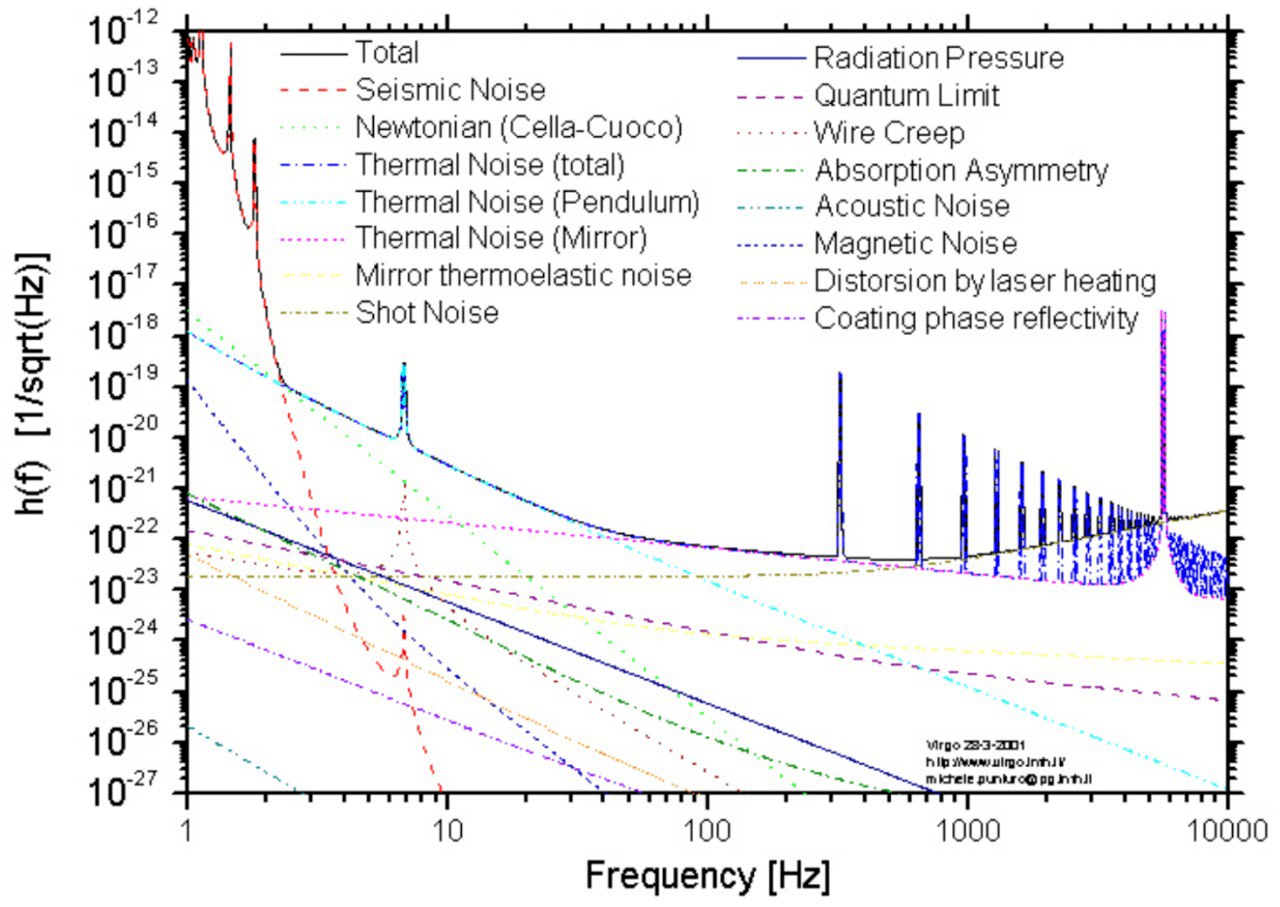
\includegraphics[scale=0.3]{noisetwo}
                        \centering
                        \caption{Noise budget}
                        \label{fig:noisetwo}
                \end{figure}

        At lower frequencies, up to 10Hz, the main contribute to the global noise
        is due to vibrations of the ground which couple to the mirror motion: it shakes the optics and produces strain signals that mask gravitational wave signals. \\
        This seismic noise could be caused by earthquakes, weather and human activity.
        To reduce the potential movements of the optical elements, an attempt is made to
        isolate the mirrors using an advanced suspension system. \\

        At frequencies where the seismic motion has been sufficiently reduced,
        between 10Hz and 500Hz, the random Brownian motion of the molecules on the surface of the mirrors and wires dominates. \\
    
        The thermal energy of the interferometer’s components induce vibrations both in the suspensions and in the mirrors.
        The nature of gravitational wave signal requires the sensitivity of the interferometric detectors
        to be extremely high in broad frequency band. \\
        Therefore, the power spectrum density of the thermal noise must be considered in the development of the detectors.
        The Fluctuation-dissipation Theorem (FDT) relates the spectrum of the thermal noise to the amount of dissipation

                \begin{equation}
                S_{n}(w) = - {{4k_bT} \over {w}} Im[H(w)]
                \end{equation}

        From this equation is possible to state that the energy of fluctuations has a frequency dependent distribution;
        $H(z)$ is the transfer function of the system, it is a mathematical function that models the device’s output, defined as

                \begin{equation}
                H(x) = {1 \over {iWZ(w)}}
                \end{equation}

        In which $Z(w)$ is the impedance of the system in the frequency domain that can be computed as the ratio
        between the Fourier components of the generalised force $\tilde F(w)$ and the response of the system $\tilde X(w)$

                \begin{equation}
                Z(w) = {{\tilde F(w)} \over {iw \tilde X(w)}}
                \end{equation}

        In the case of an harmonic oscillator, the noise spectral density is

                \begin{equation}
                S_n(w) = {{4k_bT} \over {mw}} {{{w_0}^2 \phi(w)} \over {(w^2-{w_0}^2)^2 + {w_0}^4 \phi^2(w)}}
		\end{equation} 

	Generally, thermal noise can be reduced decreasing the dissipation with monolithic suspensions and better coatings
        other than lowering the temperature using criogenic payloads as it will be done in Kagra and Einstein Telescope. \\
        Quantum mechanics limits the precision at which the test mass positions can be determined. 

        At high frequencies, photon shot noise limits the sensitivity, 
	while at low frequencies it is limited by radiation pressure.
        The photon shot noise is produced by the natural fluctuations in the rate of photons arriving at the photodiode,
        that follow a Poisson process. The noise will decrease with increasing laser power,
        recycling cavity gain, arm cavity gain, and arm length.
        The corresponding noise spectral density is

                \begin{equation}
                S_n(w) = ({{\lambda_{laser}} \over {4 \pi L}})^2 {{2 \hbar w_{laser}} \over {P}}
                \end{equation}

        Radiation pressure noise is associated with the photons from the laser striking the mirror
        and causing a force on the mirror. Of course, increasing the laser power to combat shot noise
        will actually result in an increase of radiation pressure.

                \begin{equation}
                S_n(w) =  {{32 \hbar w_{laser}P} \over {(4MLc \pi^2 f^2)^2}}
                \end{equation}

        This is an example of the Heisenberg’s Uncertainty Principle, which says that the knowledge
        of the position and the momentum of a body is restricted from the relation $\delta x \delta p \geq \hbar$. \\
        The high laser power required to determine the position of the test masses exerts
        a fluctuating radiation pressure which perturbs the test mass positions. \\
        The minimun noise level is called Standard Quantum Limit (SQL) and sets a fundamental limit
        on the sensitivity of beam detectors, contributing to the noise as

                \begin{equation}
                S_n(w) = {{2 \hbar} \over {M(\pi f L)^2}}
                \end{equation}

        Moreover, the presence of residual gas in the beam tubes would worsen the performance
        of the mirrors and of the laser; for this reason the vacuum system is maintained at a pressure
        of below $10^{-6}$Pa and the noise curve of the interferometer includes only
        the most dominant residual gas component, hydrogen, at a pressure of $10^{−7}$ Pa. \\

		\begin{figure}
                	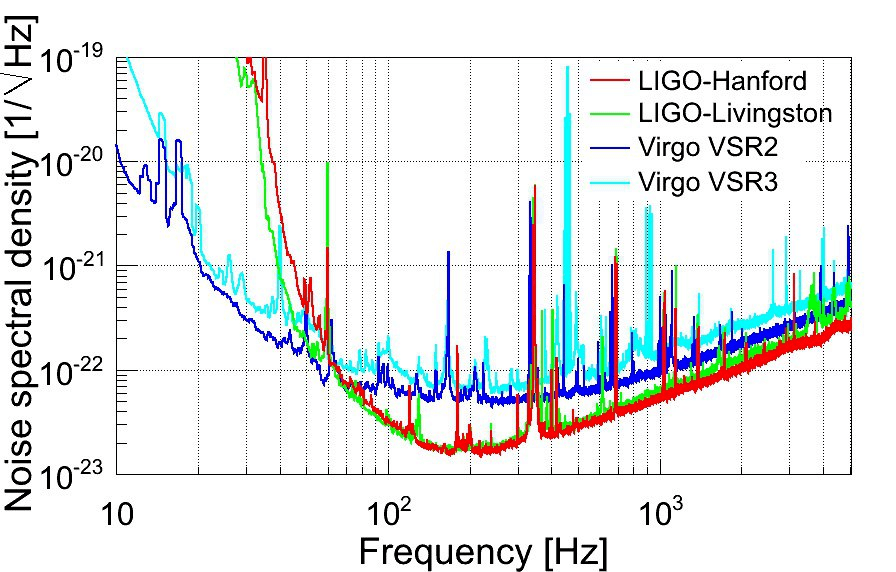
\includegraphics[scale=0.3]{noiseone}
                	\centering
                	\caption{Sensitivities of the two LIGO detectors during their S6 science run, 
				 and the Virgo detector during its VSR2 and VSR3 science runs. 
				 Each curve shows the average detector noise as a function of frequency; 
				 a signal has to be significantly above the noise to be detected reliably.}
                	\label{fig:noiseone}
                \end{figure}

\subsection{Sources}

	There are four different classes of physical sources 
	that are potential sources of gravitational waves 
	of sufficient amplitude to be detectable 
	by current or theorised gravitational wave detectors. 

\subsubsection{Coalescing compact binaries}

	Compact binary star systems, in which each member is a neutron star or black hole, 
	are currently the best understood sources of GWs. \\
	They are an ideal source for ground based GW detectors, 
	as their compactness allows their orbital separation to become 
	small enough before they merge for them to emit GWs in the detectors sensitive frequency band. \\
	If one of the components of the binary is a neutron star 
	then there may be an electromagnetic counterpart to the GW signal. \\
	The loss of energy from the system will cause the orbital radius to decay, 
	the frequency to increase, and the amplitude of the radiation to increase, 
	producing a distinctive chirp-like signal. 
	
	Eventually, the two objects will be close enough to merge together, 
	and the new single object will pulsate in an excite state as it tries to return to equilibrium. 
	This phase, known as the ringdown phase, is well-modeled as a series of quasi-normal modes. \\ 
	As the form of the gravitational radiation can be predicted allows 
	a more sensitive search to be performed: knowing the form of the signal 
	that is being search for allows powerful matched filtering techniques 
	and signal consistency tests to be used in the attempt to detect such signals.


\subsubsection{Bursts}

	A burst of gravitational waves is an event that releases a large amount 
	of gravitational energy over a very short period of time, typically less than a few seconds. \\ 
	Astrophysical events that are believed to result in a transient signal 
	include gamma ray bursts and supernovae explosion as well as the final stages of a coalescing binary. \\
	GW signal with a partially modelled or unknown waveform, 
	this may be due to unknown or complicated physics, or the source may be something totally unpredicted. 

	The matched filtering is not a useful technique to search for this type of signal, 
	as the waveform of a GW burst signal is unknown. \\
	Searches for GW bursts typically search for excess power that occurs coherently between multiple detectors. \\ 
	Even with no knowledge of the source of a GW signal, 
	it is still possible to estimate some of the source parameters. \\
	Searches for GW bursts typically give estimations of the duration, 
	amplitude and frequency of the source. 
	An estimation of the sky position is given by measuring the difference 
	in arrival time between different detectors. \\
	If the distance to the source is known, 
	perhaps through an electromagnetic counterpart, 
	then it is possible to estimate the energy of the source. 


\subsubsection{Continuous Sources}

	A periodic source is a source that emits at constant or nearly constant frequency.
	The prototypical source of continuous GWs is high frequency rotating neutron stars 
	with a non-axial deformation or low frequency binary systems 
	composed of white dwarfs or black holes far from merger. \\
	These sources should be present throughout the operational lifetime of a detector, 
	so the greater the observation time, the better the sensitivity to periodic sources becomes. 

	Spinning neutron stars will lose energy and spin down over time, 
	and this energy loss is due to a number of different mechanisms, 
	including emission of gravitational radiation. \\
	To emit a continuous GW with characteristic amplitude, 
	a neutron star must have a non-axisymmetry in the crust. 
	The radiation amplitude is proportional to the crucial parameter $\epsilon$, 
	the fractional asymmetry that is proportional to the mass of the bump on the surface.\\
	As neutron stars emit electromagnetic radiation, 
	it is possible to target searches of GWs for neutron stars with positions, 
	frequencies and spin-downs known from X-ray, radio and gamma-ray observations. 
	Examples are the Crab and Vela pulsars. 

	Continuous GWs have not yet been detected, 
	but current searches have produced upper limits for their emission. \\
	Upgraded interferometers in LIGO could set an upper limit on  
	$\epsilon$ of order $10^{-6}$ for sources at $\sim10$ kpc, 
	and explain how a neutron star can be distorted to give a value of $\epsilon$ that is interesting as a GW source. \\
	Whatever the mechanism generating the distortion, 
	it is clear that  $\epsilon$ will be small,
	so that $h \sim 10^{-24}$ or smaller, which is quite weak. \\
	Measuring these waves will require
	coherently tracking their signal for a large number of wave cycles, 
	which is actually quite difficult, 
	since the signal is strongly modulated by the Earth’s rotation and orbital motion.

	Searching for periodic GWs means demodulating the motion of the detector, 
	a computationally intensive problem since the modulation is different for every sky position. 
	Unless one knows in advance the position of the source, 
	one needs to search over a huge number of sky position "error boxes”.

\subsubsection{Stochastic background}

	Stochastic backgrounds are “random” GWs, 
	arising from a  number of sources that overlap 
	in time and frequency that are not individually resolvable. \\

	The sum of the signals at any given time and frequency will have 
	a random pattern that may be analyzed statistically but not predicted precisely. \\
	A particularly interesting source of stochastic waves is the dynamics of the early Universe, 
	which could produce an all-sky GW background, 
	similar to the cosmic microwave background. \\
	However, to measure waves from this epoch, 
	we would need much more sensitive detectors than the ground-based interferometers available.
	
	Stochastic backgrounds are usually idealized as being stationary, 
	isotropic and homogeneous and because of their random nature they look just like noise.	\\
	Another possible background could come from astrophysical sources. 
	These possible sources include a population of rotating neutron stars 
	and a population of white dwarf binaries that would be important mostly for a space-based interferometers such as LISA 

%----------------------------------------------------------------------------------------------------------------------------------------------------------------------------------------------------------
\chapter{Tecnical stuff}

\section{Signal to noise ratio}

\section{p-value}

\section{Template Bank}

\section{Coincident and coherent research}

\section{Injections}


%----------------------------------------------------------------------------------------------------------------------------------------------------------------------------------------------------------
\chapter{Gravitational wave observation so far}

\section{O1}

\section{O2}

\subsection{Gamma Ray Burst}

\section{O3a}
%----------------------------------------------------------------------------------------------------------------------------------------------------------------------------------------------------------
\chapter{Black hole-neutron star binaries}



\section{Evolution of Black Hole-Neutron Star mergers}



\subsection{Tidal disruption model}




\section{Electromagnetic Counterpart of a Black Hole-Neutron Star Binary Merger}


%----------------------------------------------------------------------------------------------------------------------------------------------------------------------------------------------------------
\chapter{My contribution to gravitational dave data analysis during O3}

\section{Bank Tests}

\section{O3 offline pyGRB analysis}

\subsection{GRB190425089}

\subsection{GRB190627A}

\subsection{GRB190728271}

\section{PyCBC O3 HL C00 data preliminary runs}

\subsection{Chunk 29}

%--------------------------------------------------------
\chapter{Conclusions}


\backmatter
\cleardoublepage

\phantomsection % Give this command only if hyperref is loaded \addcontentsline{toc}{chapter}{\bibname}

\begin{thebibliography}{100}
   \bibitem[nome]{riferimento}
\end{thebibliography}

\end{document} 

